\documentclass[runningheads]{llncs}
\usepackage[utf8]{inputenc}
\usepackage[english,vietnamese]{babel}  
\usepackage{amsmath,amssymb,amsfonts}
\usepackage{graphicx}
\usepackage{textcomp}
\usepackage{xcolor}
\usepackage{hyperref}
\usepackage{tabularx}
\usepackage{multirow}
\usepackage{multicol}
\usepackage{array}
\usepackage[table,xcdraw]{xcolor}
\usepackage{placeins}
\usepackage{tcolorbox}
\usepackage{longtable}
\usepackage{array}  
\usepackage{verbatim}
\usepackage{enumitem}
\usepackage{float}
\usepackage{caption}
\usepackage{ragged2e}
\tcbuselibrary{breakable}
\usepackage[english,vietnamese]{babel}
\addto\captionsvietnamese{
  \renewcommand{\tablename}{Table}
}
\addto\captionsvietnamese{
  \renewcommand{\abstractname}{Abstract}
}
\addto\captionsvietnamese{
  \renewcommand{\refname}{References}
}
\addto\captionsvietnamese{\renewcommand{\figurename}{Figure}}
% Define BibTeX for consistency
\def\BibTeX{{\rm B\kern-.05em{\sc i\kern-.025em b}\kern-.08em
    T\kern-.1667em\lower.7ex\hbox{E}\kern-.125emX}}

\AtBeginDocument{\justifying}
\begin{document}

\title{Integrating RAG with LLMs for Early Childhood Mental Health Support}
\titlerunning{Integrating RAG with LLMs for Early Childhood Mental Health Support}

\author{Thanh Nguyen Van Quoc\inst{1} \and
Hao Nguyen Thi Bich\inst{2} \and
Nhut Nguyen Minh\inst{3} \and
Thuan Nguyen Dinh\inst{4}}
\authorrunning{Nguyen V.Q. Thanh, Nguyen T.B. Hao, Nguyen M. Nhut, Nguyen D. Thuan}


\institute{Faculty of Information Systems, University of Information Technology - Vietnam National University, Ho Chi Minh City, Vietnam\\
\email{\{21521447@gm.uit.edu.vn, 21522049@gm.uit.edu.vn, nhutnm.17@grad.uit.edu.vn, thuannd@uit.edu.vn\}}}

\maketitle

\begin{abstract}
Currently, the need for psychological health as well as parents’ concerns about the rate of development of children is very high due to the growing number of cases of autism, Autism Spectrum Disorders (ASD), developmental delays have been discovered in recent years. However, most people are not well aware or well-gathered about this issue. Therefore, parents or relatives of the child have not yet given a correct objective assessment of these diseases. The use of the RAG framework, in conjunction with LangChain and using a Large Language Model (LLM) will help people learn and receive better results about mental health-related diseases and developmental milestones that children under 6 years old need to achieve.
\end{abstract}

\section{Introduction}
\label{sec:introduction}
With the continuous development of machine learning and deep learning, AI has been a powerful assistant in supporting people in most areas. The field of child mental health and development assessment is chosen by the team to learn, study the uses and challenges that an RAG, LangChain and LLM architecture can bring and encounter.

Our research objective is to apply the Retrieval-Augmented Generation framework (RAG) in combination with LangChain technology and outstanding LLM models for Vietnamese data. The aim is to assess the reliability and efficiency of these models when applied to the field of pediatric mental health and development. Selected LLM models include \texttt{Viet-Mistral/Vistral-7B-Chat}, \texttt{SeaLLMs/ SeaLLMs-v3-7B-Chat}, \texttt{vilm/vinallama-7b-chat}, and \texttt{vietgpt/dama-2-7b-chat}. Despite differences in model parameters, this study aims to assess the suitability of each model with the Vietnamese dataset, especially when using a relatively small amount of data to fine-tune. To evaluate model quality, we will use indicators such as METEOR, ROUGE, and Cosine Similarity.


\section{Related Works}
\label{sec:Related Works}
Kailai Yang \cite{b1} presented a paper on the integration of mental health analysis and Llama. The authors argued that Large Language Models (LLMs), particularly Llama, and their fine-tuning could significantly improve precision and clarity in predicting mental health conditions from social media data. Although LLMs such as ChatGPT and GPT-4 show good performance, they still have limitations in providing solutions and empathetic analysis based on user or client input. Therefore, fine-tuning these models with data from social networks has proven their strong generalization ability for a variety of tasks, while maintaining the quality of explanations close to human-level reasoning.

Albert Q. Jiang\cite{b2} introduced the Mistral 7B model, an LLM based on the LLaMA architecture, with 7 billion parameters designed to optimize performance and efficiency while still delivering impressive results. According to the authors, Mistral 7B outperforms the open 13B model (Llama 2) and the 34B model (Llama 1) across various benchmarks such as reasoning, mathematics, and code generation. The Grouped-Query Attention (GQA) and Sliding Window Attention (SWA) mechanisms played a crucial role in improving speed and reducing costs during training and fine-tuning. Viet-Mistral/Vistral-7B-Chat, a multi-turn conversational LLM, was created by fine-tuning the Vietnamese dataset with the proposal to extend the tokenizer for better support of the Vietnamese language.

Quan Nguyen\cite{b3} introduced Vinallama, a large language model of Vietnam based on LLAMA-2, enhanced with more than 800 billion additional training notification codes. The model shows strong fluency in Vietnamese and deep understanding of local culture. Adjusted by 1 million bilingual patterns (English-English), Vinallama-7B-Chat achieved advanced results on important NLP benchmarks of Vietnam such as VLSP, Vmlu and Vicuna benchmarks. This emphasizes its ability for specialized applications in the context of Vietnam, especially in scenarios based on dialogue. At the time the article was studied, Vinallama-7B-Chat performed quite well in the benchmark score compared to other models.

Xuan-phi Nguyen et al. \cite{b4} SEALLMS is proposed, a family of large language models specifically designed for Southeast Asian languages (SEA). These models address the language imbalance found in major LLMs by incorporating extended vocabularies, region-specific fine-tuning, and guidance links tailored to maritime languages. SEALLMS outperforms TATGPT-3.5 in several low-resource languages such as Lao, Khmer, and Burmese, demonstrating strong capabilities in multilingual guided applications and cultural awareness. We decided to include SEALLM in our research due to their flexible parameter configurations (1.5B, 7B, and 13B), as well as their continuous updates aimed at enhancing performance and language coverage over time.

Within the scope of this research, we adopt a Retrieval-Augmented Generation (RAG) architecture in combination with LangChain \cite{b5} to enhance contextual understanding for Vietnamese mental health-related queries. To enable efficient and semantically meaningful retrieval, we employ the BGE-M3 embedding model \cite{b6} to generate dense vector representations of textual data. These vectors are indexed using FAISS \cite{b8}, which allows for rapid and accurate similarity search during the retrieval phase. The retrieved context is subsequently passed to one of the selected fine-tuned LLMs (e.g., Vistral-7B-Chat, VinaLLaMA-7B, or SeaLLM-7B), enabling the system to produce contextually relevant and domain-specific responses tailored for pediatric development and mental health consultations. In addition, the research team employs evaluation metrics such as METEOR, ROUGE, and Cosine Similarity \cite{b9} \cite{b10} to assess the contextual relevance and response quality of each model. These benchmarks allow for a comprehensive comparison, enabling the selection of the most suitable model for real-world deployment in mental health and pediatric development consultation.
\section{System Architecture}
\label{sec:System Architecture}
\subsection{Overall System Design}
\label{sec:Overall System Design}
\begin{figure}[ht]
\centering

\includegraphics[width=0.95\linewidth]{bibliography/Figure/system-architech.png}
\caption{System architecture of the proposed RAG-based consulting assistant using LangChain and vinallama-2.7b-chat.}
\label{fig:architecture}
\end{figure}
The overall architecture of our system is based on the Retrieval-Augmented Generation (RAG) framework, combining a retriever and a large language model (LLM) for more accurate and context-aware responses. The system consists of two main modules: Retrieval and Generation, as illustrated in Figure~\ref{fig:architecture}.

In the \textbf{Retrieval} module, when a user submits a query, the system encodes it into a vector embedding and compares it against a pre-built FAISS vector database. This database contains vectorized embeddings of documents that were preprocessed and selected from sources related to child development and mental health. The retrieval process employs a search method using \texttt{search\_type = "similarity"} to identify documents that exhibit a high degree of relevance to the input query. Only documents that meet a predefined similarity score threshold (\texttt{score\_threshold}) are selected. These documents are then compiled into a context that is passed to the Generation module for further processing.

The \textbf{Generation} module uses a Vietnamese LLM—\texttt{vinallama-2.7b-chat} —which has been fine-tuned on domain-specific instruction data to enhance its ability to generate context-aware and helpful responses in the field of child development and mental health. The retrieved documents, along with the current prompt, context from the retrieval module, and chat history, are passed to the model as input. The model then produces a response, which is returned to the user and optionally saved for continuous interaction.

\subsection{Component Implementation Details}
\label{sec:Component Implementation Details}
\subsubsection{Vector Database Construction}\mbox{}\\
\label{sec:Vector Database Construction}

This component is responsible for transforming raw documents into vector representations that can be efficiently queried using similarity search.

The process begins by loading and parsing a collection of PDF documents containing curated knowledge related to child development and mental health. Each document is then segmented into smaller chunks using a recursive text splitter with a chunk size of 1400 characters and an overlap of 200 characters. This overlapping strategy ensures that semantic context is preserved across boundaries and improves embedding consistency.

For vectorization, we employ the BGE-M3 model from the BAAI research group. It is a multilingual, fine-tuned model optimized for dense semantic retrieval. We utilize the SentenceTransformer interface to embed both the query and the document chunks.

All embeddings are normalized and stored in a FAISS vector database. This structure enables fast approximate nearest-neighbor (ANN) search. Prior to saving, the system verifies the integrity of the index by checking the alignment between document chunks and vector entries.

To further ensure data quality and minimize retrieval noise, we test the resulting vector store with a sample query. Any failure during the process triggers an automatic cleanup of the invalid store to prevent corrupted data from affecting future interactions.

\subsubsection{LLM Fine-Tuning}\mbox{}\\
\label{sec:LLM Fine-Tuning}

This section details the methodology employed for fine-tuning various Large Language Models (LLMs) on a Vietnamese language task. The process encompasses model selection, quantization, data preprocessing, fine-tuning strategy, and evaluation.

\begin{figure}[ht]
\centering
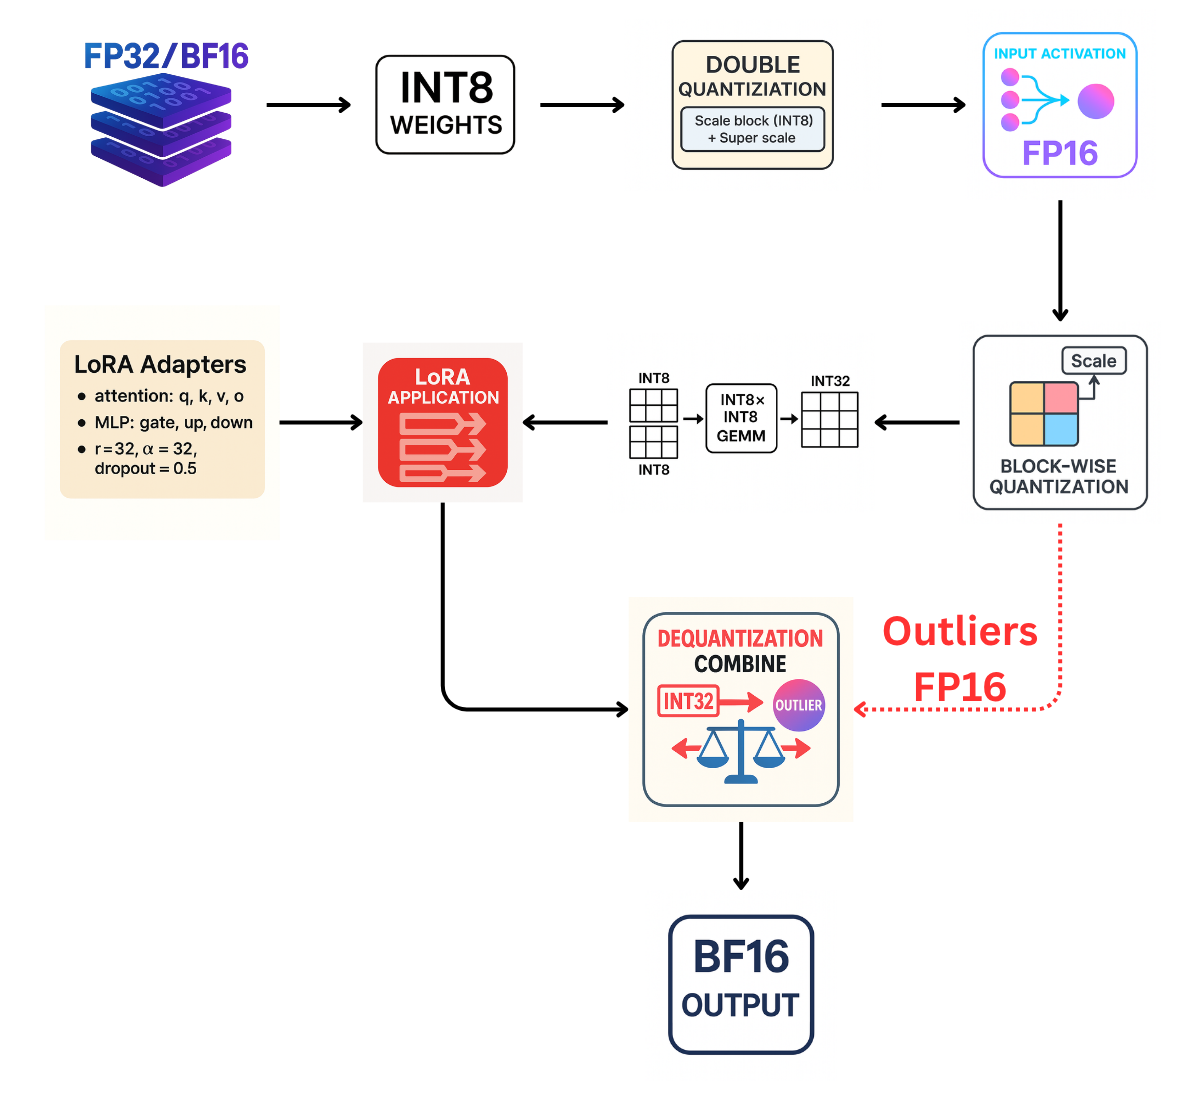
\includegraphics[width=0.95\linewidth]{bibliography/Figure/QLoRA.png}
\caption{Pineline of technique QLoRA - Quantized Low-Rank Adaptation.}
\label{fig:Pineline}
\end{figure}

\paragraph{Model Selection and Quantization}\mbox{}\\
Pretrained base models, specifically VinaLLaMA (\texttt{vilm/vinallama-7b-chat}), Vistral-7B (\texttt{Viet-Mistral/Vistral-7B-Chat}), SeaLLMs (\texttt{SeaLLMs/SeaLLMs-v3 -7B-Chat}), and Dama-2 (\texttt{vietgpt/dama-2-7b-chat}), were loaded from their respective Hugging Face repositories. To mitigate memory consumption and accelerate the training process, a strategic Post-Training Quantization (PTQ) approach was adopted using the \texttt{bitsandbytes} library. For initial single-run evaluations (Section III-B2d), models were quantized to 8-bit (int8) precision. However, for the more extensive 5-fold cross-validation (Section III-B2e), 4-bit (int4) quantization, specifically the Normalized Float 4-bit (NF4) format with \texttt{bnb\_4bit\_compute\_dtype=torch.bfloat16} and \texttt{bnb\_4bit\_use\_double\_quant =True}\cite{b7} (Figure~\ref{fig:Pineline}) , was applied. This INT4 PTQ configuration reduced the memory footprint by up to 50\% compared to FP16, enabling multiple training iterations on standard GPU hardware (e.g., NVIDIA A100). The impact of quantization was rigorously evaluated using ROUGE, METEOR, and Cosine Similarity metrics, confirming minimal degradation in response quality.

\paragraph{Low-Rank Adaptation (LoRA) Configuration}\mbox{}\\
The fine-tuning process leverages Low-Rank Adaptation (LoRA) \cite{b8} for parameter-efficient fine-tuning. A LoRA rank (\texttt{r}) of \textbf{32} was chosen as a balance between model adaptability and computational overhead, a common practice providing sufficient capacity for adaptation without an excessive increase in trainable parameters. The LoRA alpha (\texttt{lora\_alpha}) was also set to 32, and a dropout rate (\texttt{lora\_dropout}) of 0.5 was applied to LoRA layers to prevent overfitting.

To effectively adapt the models, LoRA was applied to a comprehensive set of target modules within the transformer architecture. These include:
\begin{itemize}
    \item \textbf{Attention Mechanism Modules}: \texttt{q\_proj} (query projection), \texttt{k\_proj} (key projection), \texttt{v\_proj} (value projection), and \texttt{o\_proj} (output projection). Targeting these modules allows the model to refine how it weighs and combines information from different parts of the input sequence, crucial for understanding context and relationships.
    \item \textbf{Feed-Forward Network (FFN) Modules}: \texttt{gate\_proj} (gating projection in SwiGLU/GeGLU variants), \texttt{up\_proj} (upscaling projection in FFN), and \texttt{down\_proj} (downscaling projection in FFN). Adapting these layers enables the model to learn more complex, task-specific feature transformations.
\end{itemize}
This selection aims to imbue the model with task-specific knowledge while largely preserving its pretrained general language understanding capabilities by only updating the low-rank decomposition matrices.

\paragraph{Data Preprocessing}\mbox{}\\
Rigorous data preprocessing was conducted to ensure the quality and consistency of the training dataset:
\begin{enumerate}
    \item \textbf{Text Normalization}: All text data (both instructions and responses) was converted to lowercase. Punctuation was removed to reduce noise and focus on lexical content. Vietnamese word tokenization was performed using the \texttt{underthesea} library.
    \item \textbf{Duplicate and Near-Duplicate Removal}: To prevent data leakage and improve model generalization, a fuzzy matching technique was employed. The \texttt{thefuzz} library (specifically, \texttt{fuzz.ratio}) was used to calculate the similarity between all pairs of input instructions and, separately, all pairs of output responses. Records where either the input or output exhibited a similarity score greater than a specified threshold (0.9, i.e., 90\% similarity) with another record were removed, keeping only the first occurrence. This step helps ensure a more diverse and less redundant training set.
    \item \textbf{Instruction-Response Coherence (Optional but mentioned in original thought process)}: Initially, consideration was given to filtering instruction-response pairs based on their cosine similarity using a pretrained embedding model. Pairs with similarity scores below a threshold (e.g., 0.9) would be removed to eliminate noisy or inconsistent samples. However, the primary implemented filtering focused on fuzzy matching of inputs and outputs separately as described above.
\end{enumerate}

\paragraph{Single-Run Evaluation}\mbox{}\\
\label{sec:single_run_eval}Before proceeding to full cross-validation, an initial single-run fine-tuning and evaluation was performed for each model. The preprocessed dataset was split into a training set (80\%) and an evaluation set (20\%) using a fixed \texttt{random\_state} for reproducibility. Models were fine-tuned using the LoRA configuration and int8 quantization as described above. The primary purpose of this step was to obtain a preliminary assessment of each model's performance and to debug the training pipeline.

\paragraph{5-Fold Cross-Validation}\mbox{}\\
\label{sec:cross_validation_eval}To robustly assess generalization performance and mitigate potential biases from a single train-test split, a 5-fold cross-validation strategy was employed. The entire preprocessed dataset (after fuzzy duplicate removal) was divided into five mutually exclusive folds. For each iteration, one fold served as the evaluation set, while the remaining four folds were combined to form the training set. Fine-tuning was performed independently for each of the five iterations using the LoRA configuration and int4 quantization. This approach provides a more reliable estimate of model performance across different subsets of the data.

\paragraph{Evaluation Metrics}\mbox{}\\
During 5-fold cross-validation, the \textbf{Cosine Similarity} metric was adopted as the primary criterion for selecting the best-performing fold. This semantic metric quantifies the similarity between the predicted and reference answers by computing the angular distance between their sentence embeddings. Embeddings were generated using the \texttt{BAAI/bge-m3} model from Sentence Transformers \cite{b10}. The fold with the highest average Cosine Similarity across validation samples was considered the most semantically aligned with human-labeled references and thus selected for final evaluation and analysis.

\vspace{0.8em}

\noindent \textbf{\textit{Cosine Similarity}}\\

\textbf{Formula:}

\begin{equation}
\text{CosineSim}(X, Y) = \frac{\sum_{i=1}^{n} X_i \cdot Y_i}{\sqrt{\sum_{i=1}^{n} X_i^2} \cdot \sqrt{\sum_{i=1}^{n} Y_i^2}}
\end{equation}

\textbf{Explanation:}
\begin{itemize}
  \item $X = (X_1, X_2, \dots, X_n)$ and $Y = (Y_1, Y_2, \dots, Y_n)$ are the vector representations of the candidate and reference texts, respectively.
  \item $X_i$ and $Y_i$ are the $i$-th components of vectors $X$ and $Y$ (e.g., embedding values).
  \item The numerator is the dot product between $X$ and $Y$.
  \item The denominator is the product of the Euclidean norms (magnitudes) of $X$ and $Y$.
\end{itemize}

\textbf{Interpretation:}

Cosine similarity measures the angle between two vectors in a high-dimensional space. It captures the semantic closeness between two texts regardless of their length. The score ranges from:
\begin{itemize}
  \item $1$: the vectors point in the same direction (perfect match),
  \item $0$: the vectors are orthogonal (no similarity),
  \item $-1$: the vectors are in opposite directions (rare in non-negative text embeddings).
\end{itemize}

All metrics were calculated using the \texttt{evaluate} library. For cross-validation, metrics were averaged across the five folds.

\paragraph{Best Model Selection and Merging}\mbox{}\\
Based on the average cross-validation results, particularly prioritizing Cosine Similarity, the best performing fold's adapter weights were selected for each base model. These LoRA adapters were then merged into their respective full-precision (BF16) base models to create a fine-tuned, standalone model. This merged model represents the final fine-tuned version intended for subsequent deployment or conversion.

\paragraph{GGUF Conversion for Ollama Deployment}\mbox{}\\
\label{sec:gguf_conversion}As a final step towards practical deployment, the merged fine-tuned models (in BF16 format) are intended to be converted to the GGUF (GPT-Generated Unified Format). This format is optimized for efficient inference on CPU and GPU, and is widely supported by platforms such as Ollama, facilitating local execution and broader accessibility of the fine-tuned models. The conversion process typically involves scripts provided by projects like \texttt{llama.cpp}.

\subsubsection{Integration with RAG and LangChain}

The final system was fully implemented by integrating the RAG (Retrieval-Augmented Generation) architecture with the LangChain framework, and deploying it as a production-ready chatbot using Ollama and FastAPI. Workflow of the system is shown in Figure~\ref{fig:architecture}.

\noindent\textbf{User Interaction via API Endpoint:}
The user submits a query to the API endpoint. This query is passed into the retrieval pipeline, which uses FAISS to identify the most semantically similar document chunks from the knowledge base, previously encoded using the BGE-M3 model.

\noindent\textbf{Retrieval Phase:}
The retriever searches using \texttt{search\_type = similarity} with $k$ and a \texttt{score\_threshold}. Only documents that satisfy the semantic similarity threshold are used to construct the context for the model.

\subsubsection*{System Prompt Template (Vietnamese)}\mbox{}\\

This component defines the system message that constrains the assistant’s behavior. It instructs the model to act as a pediatric mental health assistant replying exclusively in Vietnamese. The prompt includes explicit rules for:
\begin{itemize}
    \item Handling age-specific recommendations using the current date (\texttt{\{current\_date\}}).
    \item Providing clinic contact information when requested (with placeholders for phone/address).
    \item Ensuring factual, empathetic, and age-appropriate answers.
\end{itemize}
It also emphasizes priority of the provided \texttt{\{context\}} and allows fallback to pretrained knowledge only if aligned with the child’s developmental age. The prompt is injected using the \texttt{<|im\_start|>} and \texttt{<|im\_end|>} tags for compatibility with instruction-tuned LLMs.



\subsection{Dataset}

The dataset used in this research comprises two main types: 
\begin{enumerate}
    \item A conversational dataset used to train chatbot models.
    \item A document dataset used for knowledge retrieval and context injection within the RAG pipeline.
\end{enumerate}
\subsubsection*{1. Conversational Dataset for Chatbot}

This dataset was designed to support instruction-based training of Vietnamese LLMs. It consists of natural language dialogues relevant to concerns raised by parents at pediatric mental health clinics.

\begin{enumerate}
    \item \textbf{Internal Dataset:} This dataset was manually collected from real conversations on social platforms such as TikTok, Zalo, and Facebook, between parents and psychologists at a children's psychology clinic in Ho Chi Minh City. Key topics include:
    \begin{itemize}
        \item Greetings and consultation openings
        \item Developmental milestones
        \item ASQ-3 screening instructions
        \item Solutions and concerns regarding ASD or developmental delays
    \end{itemize}
    All entries were reviewed and filtered by clinical psychologists for relevance and quality.

    \item \textbf{Collected Dataset:} This dataset was constructed by extracting user queries related to child development and mental health using the Google Suggest API. The resulting keywords were clustered into topics matching the internal dataset and were validated by psychologists.

    \item \textbf{Merged Dataset:} The internal and collected datasets were combined to form high-quality instruction–response pairs, allowing the chatbot to generate both natural and professional replies.
\end{enumerate}

\begin{enumerate}[label=(\alph*)]
\item Example Dataset: 
An example data entry follows the seq2seq JSON format:

\begin{verbatim}
{
  "instruction": "Câu chào hỏi",
  "input": "Chào, cho mình hỏi?",
  "output": "Bạn cần mình giúp gì nào?"
}
\end{verbatim}

\item Number of Attributes: 
Each record contains three key-value pairs:
\begin{itemize}
    \item \texttt{instruction}: the purpose or theme of the conversation
    \item \texttt{input}: the user's question
    \item \texttt{output}: the chatbot's expected response
\end{itemize}

\item Dataset Size: 
\begin{itemize}
    \item Number of files: 4 (General Chatbot, ASD, Development, Delayed Speech)
    \item File sizes: 100KB, 45KB, 30KB, and 12KB respectively
    \item Total records: ~2,000 dialogue pairs
\end{itemize}

\item Usage: 
This dataset is used for fine-tuning and evaluating multiple Vietnamese LLMs, including:
\begin{itemize}
    \item \texttt{Viet-Mistral/Vistral-7B-Chat}
    \item \texttt{SeaLLMs/SeaLLMs-v3-7B-Chat}
    \item \texttt{vilm/vinallama-7b-chat}
    \item \texttt{vietgpt/dama-2-7b-chat}
\end{itemize}
\end{enumerate}
\subsubsection*{2. Document Dataset for Knowledge Retrieval}

This dataset comprises curated documents obtained from both public and proprietary sources, including pediatric guidelines, diagnostic manuals, and intervention documents from clinical psychologists. It supports the RAG framework by providing factual context to enhance chatbot responses.
\begin{enumerate}[label=(\alph*)]
\item Example Dataset: 
A representative document is a 10–12 page PDF outlining intervention strategies for ASD in children aged 10–12 months. The file contains textual content, tables, and clinical diagrams.

\item Number of Attributes: 
This dataset contains unstructured PDF documents; no structured attributes are defined.

\item Dataset Size: 
\begin{itemize}
    \item Number of documents: 20 PDF files
    \item Total size: approximately 35.1 MB
\end{itemize}

\item Usage: 
The documents are split into text chunks, embedded using the BGE-M3 model, and stored in a FAISS vector database. During inference, the retriever fetches relevant documents, which are injected as context into the LLM using the RAG architecture.
\end{enumerate}

\section{Results and Discussion}
\label{sec:results-discussion}

This section presents the performance evaluation of four fine-tuned large language models—SeaLLM, VinaLLaMA, Vistral, and Dama-2 on the Vietnamese mental health dialogue dataset. The evaluation was conducted using both single run testing and 5 fold cross validation, with standard metrics including ROUGE-1, ROUGE-2, ROUGE-L, METEOR, and Cosine Similarity. These metrics assess various aspects of text generation quality such as lexical overlap, fluency, semantic alignment, and vector-based similarity.

\subsection{Single-Run Evaluation}

Table \ref{tab:rouge-single-run}, \ref{tab:semantic-single-run} summarizes the evaluation scores for a single inference run across all models.

\begin{table}[H]
\centering
\caption{Single-run ROUGE Scores for All Models}
\label{tab:rouge-single-run}
\begin{tabular}{|l|c|c|c|}
\hline
\textbf{Model} & \textbf{ROUGE-1} & \textbf{ROUGE-2} & \textbf{ROUGE-L} \\
\hline
Vistral       & \textbf{0.6409} & \textbf{0.3247} & \textbf{0.4375} \\
Dama-2        & 0.6079          & 0.2874          & 0.3984          \\
VinaLLaMA     & 0.6076          & 0.2652          & 0.3891          \\
SeaLLM        & 0.6210          & 0.2679          & 0.3887          \\
\hline
\end{tabular}
\end{table} 

\begin{table}[H]
\centering
\caption{Single-run Semantic Similarity Metrics}
\label{tab:semantic-single-run}
\begin{tabular}{|l|c|c|}
\hline
\textbf{Model} & \textbf{METEOR} & \textbf{Cosine Similarity} \\
\hline
Vistral       & \textbf{0.3567} & \textbf{0.7993} \\
Dama-2        & 0.3269          & 0.7793          \\
VinaLLaMA     & 0.2958          & 0.7726          \\
SeaLLM        & 0.2989          & 0.7167          \\
\hline
\end{tabular}
\end{table}

\subsection{Cross-Validation Evaluation}

To assess the models' robustness and generalization capabilities, we applied 5-fold cross-validation. Table \ref{tab:cv-rouge}, \ref{tab:cv-semantic} shows the average scores across the folds.

\begin{table}[H]
\centering
\caption{Cross-Validation ROUGE Scores (K=5)}
\label{tab:cv-rouge}
\begin{tabular}{|l|c|c|c|}
\hline
\textbf{Model} & \textbf{ROUGE-1} & \textbf{ROUGE-2} & \textbf{ROUGE-L} \\
\hline
Vistral    & \textbf{0.6399} & \textbf{0.3158} & \textbf{0.4259} \\
Dama-2     & 0.6084 & 0.2806 & 0.3935 \\
VinaLLaMA  & 0.6104 & 0.2735 & 0.3905 \\
SeaLLM     & 0.6184 & 0.2664 & 0.3839 \\
\hline
\end{tabular}
\end{table}

\begin{table}[H]
\centering
\caption{Cross-Validation Semantic Similarity Scores (K=5)}
\label{tab:cv-semantic}
\begin{tabular}{|l|c|c|}
\hline
\textbf{Model} & \textbf{METEOR} & \textbf{Cosine Similarity} \\
\hline
Vistral    & \textbf{0.3549} & \textbf{0.7972} \\
Dama-2     & 0.3360 & 0.7757 \\
VinaLLaMA  & 0.3075 & 0.7746 \\
SeaLLM     & 0.2986 & 0.7079 \\
\hline
\end{tabular}
\end{table}

\subsection{Expert Opinion}

An expert evaluation was conducted using 21 questions collected from real-world consultations at a pediatric mental health clinic. These questions were reviewed by a specialist in child development and mental health, emphasizing clinical relevance and accuracy of responses generated by four fine-tuned AI models deployed on the Ollama platform. All models were evaluated under uniform conditions, using identical hyperparameters: temperature set at 0.5, context window size (\texttt{num\_ctx}) of 12288, and maximum prediction length (\texttt{num\_predict}) of 8192 tokens. Furthermore, each model utilized a standardized prompt clearly defining their role as an AI assistant specialized in pediatric health and mental health, tasked with providing gentle, accurate, and scientifically-based advice.

Table \ref{tab:model-response-comparison} summarizes the expert's evaluation of the responses generated by each model for a specific case involving an 18-month-old child showing signs of developmental delay. With a question Vietnamese: \textit{My child is 18 months old and can say quite a lot of words, even form three-word sentences. However, the child does not like to play with strangers. When familiar, the child laughs and plays happily. Sometimes, it feels like when I call, the child ignores me and does not}
\renewcommand{\arraystretch}{1.4}
\begin{longtable}{|>{\raggedright\arraybackslash}p{3cm}|>{\raggedright\arraybackslash}p{8cm}|>{\centering\arraybackslash}p{1.8cm}|}
\caption{Compare answers from LLM models about the case of 18-month-old children showing special signs}
\label{tab:model-response-comparison} \\
\hline
\textbf{Model} & \textbf{Response} & \textbf{Time To Response} \\
\hline
\endfirsthead

\hline
\textbf{Model} & \textbf{Response} & \textbf{Time To Response} \\
\hline
\endhead

\hline
\endfoot

Vistral-7B-Chat &  
Your child can understand longer sentences and speaks well, but is a bit shy around strangers. This is also normal because children need time to get used to new environments. You should gradually let your child interact with others and be patient during the adaptation process. & 
1.1 \\
\hline
VinaLLaMA-7B-Chat & 
At 18 months, your child can say many words and can form three-word sentences, but may not enjoy playing with strangers. When familiar, they laugh and play happily. Sometimes, they may only respond to their name without wanting to engage. It's important to practice simple conversations with them. & 
0.927 \\
\hline
Dama-2-7B-Chat & 
Hello, your child is now 18 months old and can say quite a few single words with clear intonation. However, if they do not know how to play with strangers or seem indifferent when called by name, there are some concerns about social skills that need to be monitored to ensure the child's overall development. You should continue to talk and observe your child to assess their mental and emotional health, as well as improve their communication skills with the surrounding environment if possible! Thank you for sharing this question. Wishing your beloved child always happy and healthy! &
2.207 \\
\hline
SeaLLMs-v3-7B-Chat & 
At 18 months, children typically have the ability to say about 50-70 words, so if your child can only say a few words, it is a cause for concern. You should take your child to see a language assessment specialist to ensure there are no language development issues. Regarding playing with strangers, this is also a sign to pay attention to because children at this age should start to expand their social relationships and interact with different people. You can gradually introduce your child to a small group environment to help them become more familiar and adapt. If you have any concerns about your child's development, please seek a child psychologist for detailed and specific advice for each case. &
2.703 \\
\hline

\end{longtable}

The results indicate that \textbf{SeaLLMs} model demonstrated several practical advantages over the other models. SeaLLMs consistently provided evidence-based responses, often including specific figures and statistics relevant to the child's developmental stage. The model also offered clear, actionable solutions to the problems raised in user queries, making its guidance more practical for parents. A particularly valuable feature of SeaLLMs is its frequent recommendation to seek professional help when appropriate, such as consulting a pediatrician or child psychologist. This emphasis on timely expert intervention is crucial in the context of child mental health, where early and accurate assessment by specialists can significantly impact outcomes. These strengths make SeaLLMs especially suitable for real-world deployment in pediatric mental health support, despite its slightly lower scores on some automated evaluation metrics.

A significant limitation identified across all models was their reliance on outdated medical knowledge, not fully compliant with the latest ICD-10 and ICD-11 standards. Despite extensive fine-tuning and retrieval augmentation, all models occasionally provided recommendations based on obsolete or replaced clinical guidelines. The expert highlighted the importance of continuous updates to the medical knowledge integrated into these AI systems, ensuring ongoing clinical validity and reliability of AI-generated recommendations.

\subsection{Discussion}

The comparative evaluation of the four fine-tuned models—\textbf{Vistral}, \textbf{SeaLLM}, \textbf{VinaLLaMA}, and \textbf{Dama-2}—revealed distinct differences in performance across both quantitative metrics and practical usability. According to the ROUGE, METEOR, and Cosine Similarity scores, the \textbf{Vistral} model consistently achieved the highest results, indicating its strong capability for generating semantically accurate and contextually relevant responses in Vietnamese pediatric mental health consultations. \textbf{Dama-2} and \textbf{VinaLLaMA} followed, while \textbf{SeaLLM} ranked lowest across most metrics.

However, practical expert assessment highlighted that \textbf{SeaLLM}, despite its relatively lower evaluation scores, performed admirably in real-world scenarios. The model provided coherent and relevant guidance that often met or exceeded clinical expectations, suggesting that standard text-generation metrics may not fully capture the model's effectiveness in nuanced, conversational pediatric healthcare settings.

Another important observation is that the knowledge base of the models—especially regarding up-to-date clinical standards—can be further enhanced. Missing or outdated information can be supplemented through the integration of additional high-quality and domain-specific documents, which can be ingested into the RAG retrieval system. This approach allows for continuous improvement of the assistant's knowledge without requiring complete retraining of the base language model.

In the future, the system can be further improved by combining advanced machine learning techniques and deep learning, especially techniques related to image processing and multimodal understanding. For example, taking advantage of vision large language model (Vision LLM) may allow assistance to explain and respond to visual data such as development charts or diagnostic imaging. In addition, the implementation of RAG agents, a generation strategy to enhance improvement with the decision-based decision-making.

\subsection{Acknowledgement}

This research was supported by The VNUHCM-University of Information Technology’s Scientific Research Support Fund.

We also would like to thank the experts in the field of Psychological Health for providing data and professional materials, especially the Tam Ly Nhi Dong Clinic for supporting the research team in authenticating and consolidating professional knowledge for the RAG system.

Furthermore, we are grateful to the open-source community, including Hugging Face, LangChain, and FAISS, for providing powerful tools and language models that greatly facilitated the implementation and evaluation of our system. We also appreciate the contributions of the Ollama, FastAPI and ngrok projects, which enabled the efficient deployment of our chatbot.

\begin{thebibliography}{9}
\bibitem{b1} Yang, K., Zhang, T., Kuang, Z., Xie, Q., Huang, J., Ananiadou, S.: MentaLLaMA: Interpretable Mental Health Analysis on Social Media with Large Language Models. arXiv preprint arXiv:2309.13567v3 (2024)

\bibitem{b2} Jiang, A.Q., Sablayrolles, A., Mensch, A., Bamford, C., Chaplot, D.S., de las Casas, D., Bressand, F., Lengyel, G., Lample, G., Saulnier, L., Lavaud, L.R., Lachaux, M.-A., Stock, P., Le Scao, T., Lavril, T., Wang, T., Lacroix, T., El Sayed, W.: Mistral 7B: Towards Efficient and High-Performance Language Models. arXiv preprint arXiv:2302.13971 (2023)

\bibitem{b3} Nguyen, Q., Pham, H., Dao, D.: VinaLLaMA: LLaMA-based Vietnamese Foundation Model. arXiv preprint arXiv:2312.11011v1 (2023)

\bibitem{b4} Nguyen, X.-P., Zhang, W., Li, X., Aljunied, M., Hu, Z., Shen, C., Chia, Y.K., Li, X., Wang, J., Tan, Q., Cheng, L., Chen, G., Deng, Y., Yang, S., Liu, C., Zhang, H., Bing, L.: SeaLLMs: Large Language Models for Southeast Asia. arXiv preprint arXiv:2312.16934v2 (2023)

\bibitem{b5} Gao, Y., Xiong, Y., Gao, X., Jia, K., Pan, J., Bi, Y., Dai, Y., Sun, J., Wang, M., Wang, H.: Retrieval-Augmented Generation for Large Language Models: A Survey. arXiv preprint arXiv:2312.10997v5 (2024)

\bibitem{b6} Hebert, L., Golab, L., Poupart, P., Cohen, R.: FedFormer: Contextual Federation with Attention in Reinforcement Learning. [Unpublished manuscript]

\bibitem{b7} Dettmers, T., Pagnoni, A., Holtzman, A., Zettlemoyer, L.: QLoRA: Efficient Finetuning of Quantized LLMs. arXiv preprint arXiv:2305.14314v1 (2023)

\bibitem{b8} Hu, E.J., Shen, Y., Wallis, P., Allen-Zhu, Z., Li, Y., Wang, S., Wang, L., Chen, W.: LoRA: Low-Rank Adaptation of Large Language Models. arXiv preprint arXiv:2106.09685 (2021)

\bibitem{b9} Lakatos, R., Pollner, P., Hajdu, A., Joó, T.: Investigating the Performance of Retrieval-Augmented Generation and Fine-Tuning for the Development of AI-Driven Knowledge-Based Systems. arXiv preprint arXiv:2403.09727v1 (2024)

\bibitem{b10} Steck, H., Ekanadham, C., Kallus, N.: Is Cosine-Similarity of Embeddings Really About Similarity? arXiv preprint arXiv:2403.05440v1 (2024)

\bibitem{b11} Li, H., Li, X., Hu, P., Lei, Y., Li, C., Zhou, Y., Zhou, Y.: Boosting Multi-modal Model Performance with Adaptive Gradient Modulation. arXiv preprint arXiv:2308.07686 (2023)

\bibitem{b12} Lin, C.-Y.: ROUGE: A Package for Automatic Evaluation of Summaries. In: Proceedings of the Workshop on Text Summarization Branches Out (WAS 2004), Post-Conference Workshop of ACL 2004, Barcelona, Spain (2004)

\bibitem{b13} Banerjee, S., Lavie, A.: METEOR: An Automatic Metric for MT Evaluation with Improved Correlation with Human Judgments. In: Proceedings of the ACL Workshop on Intrinsic and Extrinsic Evaluation Measures for Machine Translation and/or Summarization, Ann Arbor, Michigan, pp. 65--72 (2005)


\end{thebibliography}

\end{document}